% ------------------------------------------------------------------------
% file `ad-complogic-report-exercise-4-exercise-body.tex'
%
%     exercise of type `exercise' with id `4'
%
% generated by the `exercise' environment of the
%   `xsim' package v0.10 (2017/09/19)
% from source `ad-complogic-report' on 2017/11/22 on line 232
% ------------------------------------------------------------------------
^^I^^IОтримати МДНФ перемикальної функції, що задана діаграмою Вейча (рис.~\ref{fig:task4-veitch-diagram}). Для мінімізації застосувати метод Квайна\nbspthin —\nbspthin МакКласкі. Перемикальну функцію реалізувати в елементному базисі АБО---НЕ.
^^I^^I
^^I^^I\begin{figure}[!htbp]
^^I^^I\centering
^^I^^I^^I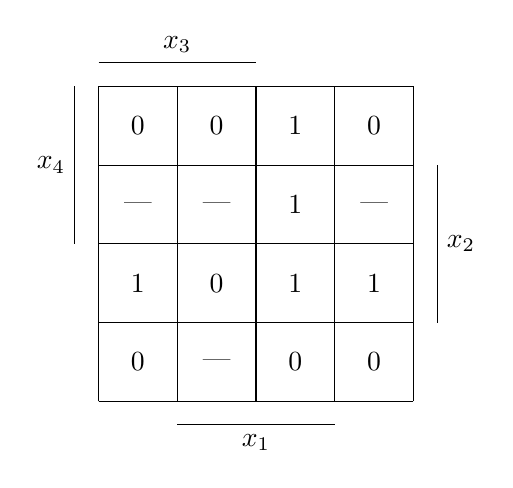
\begin{tikzpicture}
^^I^^I^^I^^I\draw (0,0) grid (4,4);
^^I^^I^^I^^I\node at (0.5,0.5){0};
^^I^^I^^I^^I\node at (1.5,0.5){—};
^^I^^I^^I^^I\node at (2.5,0.5){0};
^^I^^I^^I^^I\node at (3.5,0.5){0};

^^I^^I^^I^^I\node at (0.5,1.5){1};
^^I^^I^^I^^I\node at (1.5,1.5){0};
^^I^^I^^I^^I\node at (2.5,1.5){1};
^^I^^I^^I^^I\node at (3.5,1.5){1};
^^I^^I^^I^^I
^^I^^I^^I^^I\node at (0.5,2.5){—};
^^I^^I^^I^^I\node at (1.5,2.5){—};
^^I^^I^^I^^I\node at (2.5,2.5){1};
^^I^^I^^I^^I\node at (3.5,2.5){—};
^^I^^I^^I^^I
^^I^^I^^I^^I\node at (0.5,3.5){0};
^^I^^I^^I^^I\node at (1.5,3.5){0};
^^I^^I^^I^^I\node at (2.5,3.5){1};
^^I^^I^^I^^I\node at (3.5,3.5){0};
^^I^^I^^I^^I
^^I^^I^^I^^I\draw (0,4.3) --node[midway, above]{$x_3$} (2,4.3);
^^I^^I^^I^^I\draw (-0.3,4) --node[midway, left]{$x_4$} (-0.3,2);
^^I^^I^^I^^I\draw (1,-0.3) --node[midway, below]{$x_1$} (3,-0.3);
^^I^^I^^I^^I\draw (4.3,1) --node[midway, right]{$x_2$} (4.3,3);
^^I^^I^^I\end{tikzpicture}
^^I^^I\caption{Діаграма Вейча заданої перемикальної функції}
^^I^^I\label{fig:task4-veitch-diagram}
^^I^^I\end{figure}
^^I^^I
